\documentclass{report}
\usepackage{amsmath}
\usepackage{amssymb}
\usepackage{amsthm}
\usepackage{hyperref}
\usepackage{mathrsfs}
\usepackage{listings}
\usepackage{tikz}

% Formatting help:
% https://www.scribendi.com/advice/format_a_scientific_paper.en.html

% Theorems
\theoremstyle{definition}
\newtheorem{ax}{Axiom}
\newtheorem{defn}{Definition}

\theoremstyle{plain}
\newtheorem{thm}{Theorem}

% Nice tables
\renewcommand{\arraystretch}{1.3}

% Rust listings
\lstdefinelanguage{Rust}{
	morekeywords={enum,use,extern,crate,impl,fn,match,if,else,for,while,
	              loop,pub,struct},
	classoffset=1,
	morekeywords={self,Some,None},
	keywordstyle=\color{red},
	classoffset=2,
	morekeywords={u64,Option},
	keywordstyle=\color{green!50!black},
	classoffset=0,
	sensitive=true,
	morecomment=[l]{//},
	morecomment=[l][\color{magenta}]{\#},
	morecomment=[s]{/*}{*/},
	morestring=[b]",
}

\lstset{
	language=Rust,
	backgroundcolor=\color{gray!25},
	basicstyle=\tt\tiny,
	captionpos=b,
	commentstyle=\color{blue},
	frame=single,
	keywordstyle=\color{orange},
	numbers=left,
	numbersep=5pt,
	numberstyle=\tiny\color{brown},
	rulecolor=\color{gray},
	stepnumber=5,
	stringstyle=\color{red},
	tabsize=4,
}

\title{A Concurrent Implementation of the Randomized Condorcet Voting System}
\author{Pierre Colin}
\date{}

\begin{document}
\maketitle

\begin{abstract}
TODO
\end{abstract}

\chapter{Democracy and election systems}
TODO

\section{Formalization of an election}
In a general election, the term \emph{alternative} is preferred to candidate as
the latter only applies well to human alternatives. The set of alternatives
will be noted $V$ because of an analogy with graph theory which will be made
clear in the next chapter.

\subsection{Naive ballots}
There are lots of ways to formalize ballots in an election. The one used here
relies on duels: a ballot will be a binary relation on $V$. In practice, an
elector would be given a grid where rows and columns are alternatives, and for
all squares, they would have to indicate which alternative they prefer. Of
course, the diagonal of the grid would have to be full of ties, and it would
have to be antisymmetric in the sense that a win of $x$ over $y$ in one square
needs to be reported as a loss of $y$ over $x$ in its symmetric square. As a
result, only a little below half of the grid needs to be filled, but this still
yields a ballot complexity of
$n\,\left(n\,-\,1\right) \,/\, 2\;
	=\; \underset{n\;\to\;\infty}\Theta\left(n^2\right)$
where $n\;=\;\left|V\right|$, and it would leave room for cyclical preferences.

The problem with cyclical preferences is that they open the doors to easy
scams. Consider the following: a person buys vanilla ice cream for \$1.00. The
ice cream man offers a one-cent switch of vanilla for chocolate, which the
customer accepts. The ice cream man then offers a one-cent switch of chocolate
for caramel, which the customer accepts. The ice cream man then offers a
one-cent switch of caramel for vanilla, which the customer accepts. The
customer has now paid \$1.03 for the same ice cream and may accept further
one-cent switches in the same fashion in such a way they may pay an unbounded
amount for an ice cream that is supposed to cost \$1.00.

\subsection{Strictly-preordered ballots}
To avoid cyclical preferences, the simple solution is to instead model ballots
as strict preorders over $V$. An elector has to give ranks to alternatives. An
alternative may be unranked, in which case it won't be compared to any other
alternative. The easy way to construct a strict preorder consists of giving all
ranked alternatives a range of ranks in $\mathbf N$. If we denote the unranked
property by $\varnothing$, this means constructing a function
$f:\;V\;\longmapsto\;\mathbf N^2\,\cup\,\left\{\varnothing\right\}$ such that
for all $v\;\in\;V$:
\begin{itemize}
\item if $v$ is unranked, then $f\left(v\right)\;=\;\varnothing$;
\item if $v$ is ranked, there exists $\left(a,\;b\right)\;\in\;\mathbf N^2$ such
      that $a\;\leqslant\;b$ and $f\left(v\right)\;=\;\left(a,\;b\right)$.
\end{itemize}
The alternatives can then be compared in the following way: for all
$\left(x,\;y\right)\;\in\;V^2$,
\begin{itemize}
\item if $f\left(x\right)\;=\;\varnothing$ or $f\left(y\right)\;=\;\varnothing$,
      then $x$ and $y$ are incomparable;
\item if $f\left(x\right)\;=\;\left(a_x,\;b_x\right)$ and
      $f\left(y\right)\;=\;\left(a_y,\;b_y\right)$, then $x\;<\;y$ if and only
      if $b_x\;<\;a_y$.
\end{itemize}
\begin{thm}
	The binary relation $<$ is a strict preorder over $V$.
\end{thm}
\begin{proof}
	Prove $<$ is irreflexive and transitive.
	\begin{description}
	\item[Irreflexivity:]
	Let $v\;\in\;V$. If $f\left(v\right)\;=\;\varnothing$, then $v$ is
	incomparable to itself. If $f\left(v\right)\;=\;\left(a,\;b\right)$
	with $a\;\leqslant\;b$, then we don't have $b\;<\;a$ hence we don't
	have $v\;<\;v$. In all cases, $v$ is incomparable to itself. Therefore,
	$<$ is irreflexive.
	\item[Transitivity:]
	Let $\left(x,\;y,\;z\right)\;\in\;V^3$ such that $x\;<\;y$ and
	$y\;<\;z$. Since they are pairwise comparable, they are all ranked.
	Destructure $f\left(x\right)\;=\;\left(a_x,\;b_x\right)$,
	$f\left(y\right)\;=\;\left(a_y,\;b_y\right)$ and
	$f\left(z\right)\;=\;\left(a_z,\;b_z\right)$. Combining properties on
	rank ranges and the definition of $<$ between alternatives,
	$b_x\;<\;a_y\;\leqslant\;b_y\;<\;a_z$ hence $b_x\;<\;a_z$ i.e.
	$x\;<\;z$. Therefore, $<$ is transitive.
	\end{description}
\end{proof}
By replacing all occurences of $<$ with $\leqslant$ and adding the constraint
$\forall v\;\in\;V,\;v\;\leqslant\;v$, it is possible to construct a preorder
over $V$. Preorders are a common way to model preferences, but insufficient for
modelling duels. A strict preorder property guarantees the absence of cycles,
and it is both easy to implement and yields a ballot of complexity
$n\;=\;\underset{n\;\to\;\infty}\Theta\left(n\right)$ where
$n\;=\;\left|V\right|$ which is much simpler than the naive ballot.

\section{Implementation}
Unlike what the theory suggests, the unranked property is not implemented in
the type \verb!Rank!. Instead, an unranked alternative is simply absent from
the ballot which is implemented as a \verb!HashMap<A, Rank>! where \verb!A!
denoes the generic type for alternatives. As the whole library makes use of
Rust's generics, \verb!A! requires some traits, namely \verb!std::cmp::Eq! and
\verb!std::hash::Hash!.

\subsection{Ranks}
First, implement ranks as a pair of 64-bit unsigned integers, and derive the
\verb!Debug! trait for testing purposes.
\begin{lstlisting}
#[derive(Debug)]
pub struct Rank(u64, u64);
\end{lstlisting}
However, not all pairs of 64-bit integers \verb!(a, b)! is a valid rank as the
constraint \verb!a <= b! is required. Because of that, a method \verb!new! is
needed for the type \verb!Rank! to make sure the rank given is valid.
\begin{lstlisting}
impl Rank {
    pub fn new(a: u64, b: u64) -> Option<Rank> {
        if a <= b {
            Some(Rank(a, b))
        } else {
            None
        }
    }
}
\end{lstlisting}

The trait \verb!fmt::Display! is implemented to print ranks in a pretty way.
The trait \verb!cmp::PartialEq! is implemented so that ranks never equal one
another. The trait \verb!cmp::PartialOrd! is implemented to reflect the strict
preorder that was defined in the previous section. This is done with the
following code:
\begin{lstlisting}
impl cmp::PartialOrd for Rank {
    fn partial_cmp(&self, other: &Rank) -> Option<cmp::Ordering> {
            match (self, other) {
                (&Rank(_, b), &Rank(a, _)) if b < a
                    => Some(cmp::Ordering::Less),
                (&Rank(a, _), &Rank(_, b)) if b < a
                    => Some(cmp::Ordering::Greater),
                _ => None,
            }
    }
}
\end{lstlisting}

\subsection{Ballots}
In order to be easily accessible by the client, ballots are implemented in the
root file \verb!lib.rs!. They are essentially a wrapped \verb!HashMap<A, Rank>!
with some convenient methods.
\begin{lstlisting}
pub struct Ballot<A: Hash> {
    m: HashMap<A, ballot::Rank>
}

impl <A: Hash + Eq> Ballot<A> {
    pub fn new() -> Ballot<A> {
        Ballot::<A>{ m: HashMap::<A, ballot::Rank>::new() }
    }

    pub fn insert(&mut self, x: A, a: u64, b: u64) -> bool {
        let or = ballot::Rank::new(a, b);
        match or {
            Some(r) => { self.m.insert(x, r); true },
            None => false,
        }
    }

    pub fn remove(&mut self, x: &A) -> bool {
        self.m.remove(x) != None
    }

    pub fn iter(&self) -> hash_map::Iter<A, ballot::Rank> {
        self.m.iter()
    }
}
\end{lstlisting}

The \verb!insert! method differs from the one provided by \verb!HashMap! in
that its return value indicates not the old value stored, but whether or not
the rank created is a valid one.

\chapter{The Condorcet Voting System}
The first main idea by Nicolas de Condorcet (1743--1794) is now known as the
Condorcet criterion.
\begin{ax}[Condorcet]
	If an alternative wins in one-versus-one duels against all others in an
	election, then it should be elected.
\end{ax}
Such an alternative is called a \emph{Condorcet winner}. This chapter explores
the Condorcet Voting System which is centered around this criterion.

\section{Definitions}
One-versus-one duels are typically visualized using graph theory.
\begin{defn}
	Let $V$ be the set of alternatives in the election. The \emph{duel
	graph} of the election is the oriented graph $\left(V,\;A\right)$ such
	that for all $\left(x,\;y\right)\;\in\;V^2$, the arrow
	$\overrightarrow{x\,y}$ is in $A$ if and only if more electors prefer $x$
	over $y$ than the opposite. Since it makes no sense to say that an
	alternative beats itself, duel graphs are trivially simple directed
	graphs.
\end{defn}
It may be useful to recall some theorems of graph theory which act as
interesting properties of duel graphs. Table \ref{tbl:duel_graph_vocab} shows
the correspondence between graph theory vocabulary and election system
vocabulary. Some of these correspondances are definitions; others are trivial
properties.
\begin{table}
	\centering
	\begin{tabular}{lr}
		\hline
		Graph theory & Election system \\
		\hline
		Vertice & Alternative \\
		$\overrightarrow{x\,y}\;\in\;A$ & $x$ beats $y$ \\
		$G$ is a tournament & There is no tie \\
		Source & Condorcet winner \\
		Sink & Condorcet loser \\
		\hline
	\end{tabular}
	\caption{Vocabulary of duel graphs}
	\label{tbl:duel_graph_vocab}
\end{table}
The duel graph of an election being a tournament is more likely as the number
of voters increases. Figure \ref{fig:duel_one_winner} shows a duel graph with a
unique Condorcet winner.
\begin{figure}
	\centering
	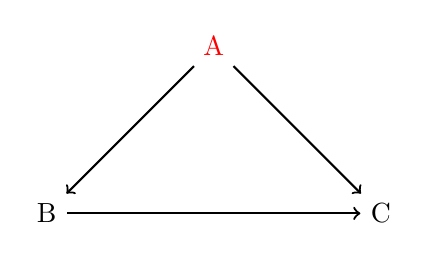
\begin{tikzpicture}[->, thick, node distance=3cm]
		\node[color=red] (A) {A};
		\node (B) [below left of=A] {B};
		\node (C) [below right of=A] {C};
		\path (A) edge (B)
		          edge (C)
		      (B) edge (C);
	\end{tikzpicture}
	\caption{A duel graph with \textcolor{red}{A} being a Condorcet winner}
	\label{fig:duel_one_winner}
\end{figure}

\begin{thm}
	A tournament has at most one source.
	\label{thm:tournament_sink}
\end{thm}
\begin{proof}
	Let $G\;=\;\left(V,\;A\right)$ be a tournament. Suppose by contradiction
	that it has two sources $x$ and $y$. Since $G$ is a tournament, exactly
	one of the arrows $\overrightarrow{x\,y}$ and $\overrightarrow{y\,x}$ is
	in $A$. Without loss of generality, assume the former. Then
	$\deg^-\left(y\right)\;>\;0$ i.e. $y$ is not a source, yielding a
	contradiction.
\end{proof}
Using all the notions presented in this section, the Condorcet method appears
to be simple: have electors express pairwise comparisons between alternatives,
build the duel graph and elect the alternative which corresponds to a sink in
the duel graph.

\section{The Condorcet paradox}
Unfortunately, there are situations in which the naive method alluded to at the
end of the previous section cannot be used. It is possible, albeit rare in
official elections, that there are zero or more than one Condorcet winners.
Figures \ref{fig:duel_no_winner} and \ref{fig:duel_two_winners} show these
situations. Note that the duel graph on figure \ref{fig:duel_two_winners} does
not contradict theorem \ref{thm:tournament_sink} because the graph is not a
tournament. The situation illustrated on figure \ref{fig:duel_no_winner} is
known as the \emph{Condorcet paradox}: even if the electors' individual
preferences are acyclical, the duel graph may be cyclical, meaning assuming
otherwise would be a fallacy of composition.
\begin{figure}
	\centering
	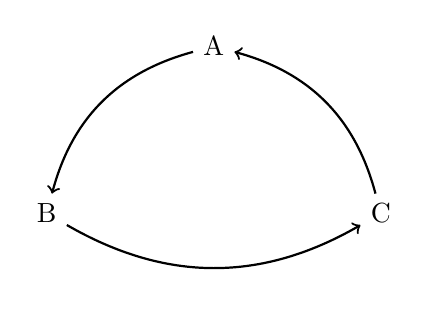
\begin{tikzpicture}[->, thick, node distance=3cm]
		\node (A) {A};
		\node (B) [below left of=A] {B};
		\node (C) [below right of=A] {C};
		\path (A) edge[bend right] (B)
		      (B) edge[bend right] (C)
		      (C) edge[bend right] (A);
	\end{tikzpicture}
	\caption{A duel graph with no Condorcet winner}
	\label{fig:duel_no_winner}
\end{figure}
\begin{figure}
	\centering
	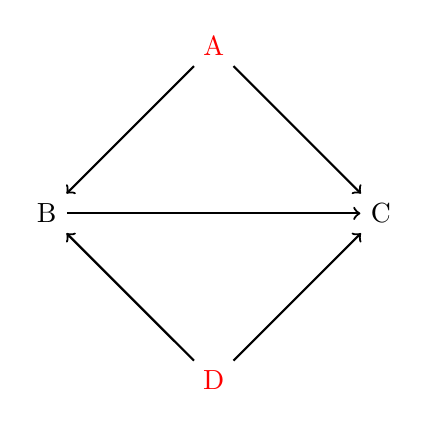
\begin{tikzpicture}[->, thick, node distance=3cm]
		\node[color=red] (A) {A};
		\node (B) [below left of=A] {B};
		\node (C) [below right of=A] {C};
		\node[color=red] (D) [below right of=B] {D};
		\path (A) edge (B)
		          edge (C)
		      (B) edge (C)
		      (D) edge (B)
		          edge (C);
	\end{tikzpicture}
	\caption{A duel graph with \textcolor{red}{A} and \textcolor{red}{D}
	         both being Condorcet winners}
	\label{fig:duel_two_winners}
\end{figure}

In these situations, an alternative method needs to be used to fill the gaps
of the Condorcet method. Several methods exist, and the one used in this
project is fairly new. However, no matter what alternative method is used, the
naive Condorcet Voting System needs to be implemented since it is an inherent
part of all of the existing alternative methods.

\section{Implementation}
TODO

\chapter{Nondeterministic winner}
Thanks to game theory, new tools allowed to find solutions to the case where no
deterministic winner can be chosen, namely mixed strategies and the minimax
theorem. The main idea is that the winner is chosen randomly according to a
probability distribution which maximizes the average elector's utility
\footnote{the game theory term for happiness}.

\section{Rock-paper-scissors}
The first observation to be made is that duel graphs are isomorphic to the
rules of the generalized rock-paper-scissors game, where vertices correspond to
decisions and arrows model comparisons between decisions. Figure
\ref{fig:rock_paper_scissors} is copied from \ref{fig:duel_no_winner} with
renamed vertices to show exactly that. The game-theory properties of
rock-paper-scissors are:
\begin{description}
\item[2 players:] two players taking decisions;
\item[Non-cooperative:] players have no interest in helping each other;
\item[Symmetric:] the payoff of a strategy only depends on the opponent's
                  strategy;
\item[Zero sum:] the winner's utility gain equals the loser's utility loss;
\item[Simultaneous:] players make decisions without knowing the decisions made
                     by their opponent;
\item[Finite:] only three decisions possible;
\item[2 outcomes:] draw or win-loss.
\end{description}
\begin{figure}
	\centering
	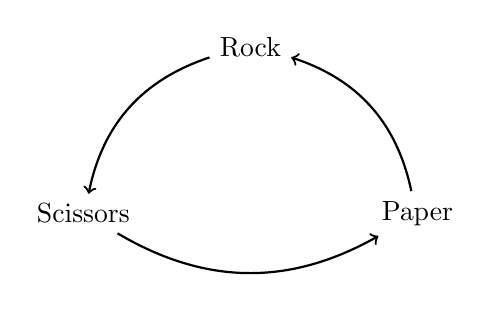
\begin{tikzpicture}[->, thick, node distance=3cm]
		\node (A) {Rock};
		\node (B) [below left of=A] {Scissors};
		\node (C) [below right of=A] {Paper};
		\path (A) edge[bend right] (B)
		      (B) edge[bend right] (C)
		      (C) edge[bend right] (A);
	\end{tikzpicture}
	\caption{The rock-paper-scissors duel graph}
	\label{fig:rock_paper_scissors}
\end{figure}
Duel graphs may thus be seen as rock-paper-scissors-like games, and the goal is
to find an optimal strategy for this game. In the case of rock-paper-scissors,
there exist strategies based on psychology, but these work only because of
human cognitive biases. They should not be used in this context. One may argue
that no particular strategy can be derived for a simultaneous game, but this
is actually false as soon as players allow themselves to play randomly.

\section{Mixed strategies}
When playing rock-paper-scissors, it turns out that the best strategy is to
play randomly. In front of such a strategy, no counter-strategy can be devised,
and the expected win frequency is always $33\,\%$.

\begin{defn}
	Consider a finite, symmetric, simultaneous game. A \emph{mixed
	strategy} is a strategy in which the player randomly picks a decision
	according to a probability distribution.

	As both players can choose between $n\;=\;\left|V\right|$ decisions,
	such strategies are modeled as random variables over $V$.
\end{defn}

For convenience, define $I\;=\;\left\{1,\;\ldots,\;n\right\}$ and let
$\begin{array}[t]{cccl}v:&I&\longrightarrow&V \\
&n&\longmapsto&v\left(n\right)\end{array}$ be a bijection between $I$ and $V$.

\subsection{Comparison}
Let $X$ and $Y$ be two mixed strategies over $V$. Intuitively, $X$ beats $Y$ if
and only if
\begin{equation}
	\mathbf P\left(\overrightarrow{X\,Y}\;\in\;A\right)\;
	\geqslant\;\mathbf P\left(\overrightarrow{Y\,X}\;\in\;A\right).
	\label{eqn:compare_distributions}
\end{equation}

Some playing around may cast light on another formalism for mixed strategies.
Denoting the duel graph as $G\;=\;\left(V,\;A\right)$, Let \[
\begin{array}[t]{cccl}
s:&V&\longrightarrow&\mathscr P\left(V\right) \\
&x&\longmapsto&\left\{y\;\in\;V\mid\overrightarrow{x\,y}\;\in\;A\right\}
\end{array}
\] be the function giving the successors of a vertice in $G$. Noting that the
game is simultaneous, $X$ and $Y$ are independent and equation
\ref{eqn:compare_distributions} becomes \[
	\sum_{x\;\in\;V}\mathbf P\left(X\;=\;x\right)\,
	\sum_{y\;\in\;s\left(x\right)}\mathbf P\left(Y\;=\;y\right)
	\;\geqslant\;
	\sum_{y\;\in\;V}\mathbf P\left(Y\;=\;y\right)\,
	\sum_{x\;\in\;s\left(y\right)}\mathbf P\left(X\;=\;x\right).
\] which can be rearranged as
\begin{equation}
	\sum_{x\;\in\;V}\sum_{y\;\in\;s\left(x\right)}\left(
	\mathbf P\left(X\;=\;x\right)\,\mathbf P\left(Y\;=\;y\right)
	\,-\,
	\mathbf P\left(Y\;=\;x\right)\,\mathbf P\left(X\;=\;y\right)\right)
	\;\geqslant\;0.
	\label{eqn:rearranged_comparison}
\end{equation}

\subsection{Mixed vectors}
Let $M\;=\;\left(m_{i,\;j}\right)_{\left(i,\;j\right)\;\in\;I^2}
\;\in\;\mathscr M_n\left(\mathbf R\right)$ be the matrix defined by \[
	\forall\left(i,\;j\right)\;\in\;I^2,\;m_{i,\;j}\;=\;
	\begin{cases}
		1\qquad\text{if }
			\overrightarrow{v\left(i\right)\,v\left(j\right)}
				\;\in\;A \\
		-1\qquad\text{if }
			\overrightarrow{v\left(j\right)\,v\left(i\right)}
				\;\in\;A \\
		0\qquad\text{otherwise}
	\end{cases}.
\]

\begin{thm}
	The matrix $M$ is skew-symmetric.
\end{thm}
\begin{proof}
	Let $\left(i,\;j\right)\;\in\;I^2$. If $i\;=\;j$, then
	$\overrightarrow{v\left(i\right)\,v\left(j\right)}\;\notin\;A$ thus
	$m_{i,\;j}\;=\;0$. Assume $i\;\neq\;j$. Since $G$ is oriented, exactly
	one of the following is true:
	\begin{enumerate}
	\item $\overrightarrow{v\left(i\right)\,v\left(j\right)}\;\notin\;A$
	      and
	      $\overrightarrow{v\left(j\right)\,v\left(i\right)}\;\notin\;A$,
	      then $m_{i,\;j}\;=\;0\;=\;-m_{j,\;i}$.
	\item $\overrightarrow{v\left(i\right)\,v\left(j\right)}\;\in\;A$
	      and
	      $\overrightarrow{v\left(j\right)\,v\left(i\right)}\;\notin\;A$,
	      then $m_{i,\;j}\;=\;1\;=\;-\left(-1\right)\;=\;-m_{j,\;i}$.
	\item $\overrightarrow{v\left(i\right)\,v\left(j\right)}\;\notin\;A$
	      and
	      $\overrightarrow{v\left(j\right)\,v\left(i\right)}\;\in\;A$,
	      then $m_{i,\;j}\;=\;-1\;=\;-m_{j,\;i}$.
	\end{enumerate}
	In all cases, $m_{i,\;j}\;=\;-m_{j,\;i}$, thus $M$ is skew-symmetric.
\end{proof}

\begin{defn}
	Let $X$ be a mixed strategy over $V$. The \emph{mixed vector} assigned
	to $X$ is \[
		\left(\mathbf P\left(X\;
				=\;v\left(i\right)\right)\right)
			_{i\;\in\;I}
		\;\in\;\mathscr M_{n,\;1}\left(\mathbf R\right).
	\]
\end{defn}

Taking equation \ref{eqn:rearranged_comparison} with
$P\;=\;\left(p_i\right)_{i\;\in\;I}$ and $Q\;=\;\left(q_i\right)_{i\;\in\;I}$
being the mixed vectors assigned to $X$ and $Y$ respectively, \[
	\sum_{i\;\in\;I}
	\sum_{\substack{j\;\in\;I \\ m_{i,\;j}\;=\;1}}
	\left(p_i\,q_j\,-\,q_i\,p_j\right)
	\;\geqslant\;0.
\] Using $M$'s skew-symmetry,
\begin{align*}
	\sum_{i\;\in\;I}
	\sum_{\substack{j\;\in\;I \\ m_{i,\;j}\;=\;1}}
	\left(p_i\,q_j\,-\,q_i\,p_j\right)
	\;&=\;
	\sum_{\substack{\left(i,\;j\right)\;\in\;I^2 \\ m_{i,\;j}\;=\;1}}
	\left(p_i\,q_j\,-\,q_i\,p_j\right) \\
	&=\;
	\sum_{\substack{\left(i,\;j\right)\;\in\;I^2 \\ m_{i,\;j}\;=\;1}}
	p_i\,q_j
	\,-\,\sum_{\substack{\left(i,\;j\right)\;\in\;I^2 \\ m_{i,\;j}\;=\;1}}
	q_i\,p_j \\
	&=\;
	\sum_{\substack{\left(i,\;j\right)\;\in\;I^2 \\ m_{i,\;j}\;=\;1}}
	p_i\,1\,q_j
	\,+\,\sum_{\substack{\left(i,\;j\right)\;\in\;I^2 \\ m_{j,\;i}\;=\;-1}}
	p_j\,\left(-1\right)\,q_i \\
	&=\;
	\sum_{\substack{\left(i,\;j\right)\;\in\;I^2 \\ m_{i,\;j}\;=\;1}}
	p_i\,1\,q_j
	\,+\,\sum_{\substack{\left(i,\;j\right)\;\in\;I^2 \\ m_{i,\;j}\;=\;-1}}
	p_i\,\left(-1\right)\,q_j.
\end{align*}
Since $\forall\left(i,\;j\right)\;\in\;I^2,\;
m_{i,\;j}\;\in\;\left\{-1,\;0,\;1\right\}$, noting $M_i$ the $i$th row of $M$,
the two sums can be merged into
\begin{align*}
	\sum_{\left(i,\;j\right)\;\in\;I^2}p_i\,m_{i,\;j}\,q_j
	\;&=\;\sum_{i\;\in\;I}\sum_{j\;\in\;I}p_i\,m_{i,\;j}\,q_j \\
	&=\;\sum_{i\;\in\;I}p_i\,\sum_{j\;\in\;I}m_{i,\;j}\,q_j \\
	&=\;\sum_{i\;\in\;I}p_i\,\left(M_i\,Q\right) \\
	&=\;\sum_{i\;\in\;I}\left(p_i\,M_i\right)\,Q \\
	&=\;\left(\sum_{i\;\in\;I}p_i\,M_i\right)\,Q \\
	&=\;\left(P^\top\,M\right)\,Q \\
	&=\;P^\top\,M\,Q \\
\end{align*}

From this observation, a preorder on mixed vectors can be defined.
\begin{defn}
	\label{defn:mixed_vector}
	Let $\mathbf P$ be the set of vectors $\left(p_i\right)_{i\;\in\;I}
	\;\in\;\mathscr M_{n,\;1}\left(\mathbf R\right)$ such that
	$\forall i\;\in\;I,\;p_i\;\geqslant\;0$ and $\sum_{i\;\in\;I}p_i\;1$.
	Introduce a binary relation $\leqslant$ over $\mathbf P$ such that for
	all $\left(P,\;Q\right)\;\in\;\mathbf P^2$,
	\[P\;\leqslant\;Q\quad\Leftrightarrow\quad P^\top\,M\,Q\;\leqslant\;0.\]
\end{defn}

By the manipulations done above, the notion of mixed vector is isomorphic to
that of mixed strategies, and the binary relation between mixed vectors is
equivalent to mixed strategies beating each other.

\begin{thm}
	The binary relation $\leqslant$ is reflexive and total.
\end{thm}
\begin{proof}
	Prove that $\leqslant$ is reflexive and transitive.
	\begin{description}
	\item[Reflexivity:] Let $P\;\in\;\mathbf P$. Since $P$ only has
		nonnegative coordinates,
		\begin{align*}
		P^\top\,M\,P
		\;&=\;\sum_{\left(i,\;j\right)\;\in\;I^2}p_i\,m_{i,\;j}\,p_j \\
		&=\;\sum_{\substack{\left(i,\;j\right)\;\in\;I^2 \\
		                    m_{i,\;j}\;=\;1}}
			p_i\,p_j
		\,-\,\sum_{\substack{\left(i,\;j\right)\;\in\;I^2 \\
		                     m_{i,\;j}\;=\;-1}}
			p_i\,p_j \\
		&=\;\sum_{\substack{\left(i,\;j\right)\;\in\;I^2 \\
		                    m_{i,\;j}\;=\;1}}
			p_i\,p_j
		\,-\,\sum_{\substack{\left(i,\;j\right)\;\in\;I^2 \\
		                     m_{j,\;i}\;=\;1}}
			p_j\,p_i \\
		&=\;0\;\leqslant\;0.
		\end{align*}
		Therefore $\leqslant$ is reflexive.
	\item[Totality:] Let $\left(P,\;Q\right)\;\in\;\mathbf P^2$. Suppose
		$P\;\leqslant\;Q$ is false. Then $P^\top\,M\,Q\;>\;0$. But
		$P^\top\,M\,Q\;=\;\left(Q^\top\,M^\top\,P\right)^\top$, and
		since this quantity is a scalar and $M$ is skew-symmetric, it
		equals $-Q^\top\,M\,P\;>\;0$ i.e. $Q^\top\,M\,P\;<\;0$ then
		$Q\;\leqslant\;P$. Therefore, $\leqslant$ is total.
	\end{description}
\end{proof}

\subsection{Maximal strategies}
The goal is now to find an \emph{optimal} mixed strategy. The minimax approach
will be useful for that. The following calculations are taken from oscar6echo's
notebook\cite{oscar6echo}. Both the minimax and maximin strategies are covered
here, although they are extremely similar.

\subsubsection{Minimax strategy}
Suppose player B wants to choose a strategy $P\;\in\;;\mathbf P$ that will
maximize its payoff, i.e. minimize A's, no matter what mixed strategy player A
plays. Since mixed strategies are barycenters of pure strategies, it is
possible to assume player A plays the optimal pure strategy. Noting $M_i$ the
$i$th row of $M$, A's expected payoff is then
\[v\;=\;\min_{P\;\in\;\mathbf P}\,\max_{i\;\in\;I}\,M_i\,P.\]
Since the maximum is equivalent to the least upper bound,
\[
	v\;=\;\min_{P\;\in\;\mathscr M_{n,\;1}\left(\mathbf R\right)}\,\min_{a\;\in\;\mathbf R}\,a
		\qquad\text{subject to}\qquad
		\begin{cases}
		\forall i\;\in\;I,\;p_i\;\geqslant\;0 \\
		\sum_{i\;\in\;I}p_i\;=\;1 \\
		\forall i\;\in\;I,\;M_i\,P\;\leqslant\;a
		\end{cases}.
\]
Merging both minima,
\begin{equation}
	v\;=\;\min_{\substack{P\;\in\;\mathscr M_{n,\;1}\left(\mathbf R\right)\\a\;\in\;\mathbf R}}\,a
		\qquad\text{subject to}\qquad
		\begin{cases}
		\forall i\;\in\;I,\;p_i\;\geqslant\;0 \\
		\sum_{i\;\in\;I}p_i\;=\;1 \\
		\forall i\;\in\;I,\;M_i\,P\;\leqslant\;a
		\end{cases}.
	\label{eqn:minimax_1}
\end{equation}
For all $\left(i,\;j\right)\;\in\;I^2$, define $m'_{i,\;j}\;=\;m_{i,\;j}\,+\,2$
so that the matrix $M'$ has only positive coordinates. Then for all $i\;\in\;I$,
\begin{align*}
	M'_i\,P\;&=\;\sum_{j\;\in\;I}m'_{i,\;j}\,p_j \\
		&=\;\sum_{j\;\in\;I}\left(m_{i,\;j}\,+\,2\right)\,p_j \\
		&=\;\sum_{j\;\in\;I}\left(m_{i,\;j}\,p_j\,+\,2\,p_j\right) \\
		&=\;\sum_{j\;\in\;I}m_{i,\;j}\,p_j\,+\,2\,\sum_{j\;\in\;I}p_j \\
		&=\;\sum_{j\;\in\;I}m_{i,\;j}\,p_j\,+\,2 \\
		&=\;M_i\,P\,+\,2.
\end{align*}
This guarantees switching from $M$ to $M'$ will only shift $a$ by 2, meaning,
for $a'\;=\;a\,+\,2$, equation \ref{eqn:minimax_1} becomes
\begin{equation}
	v'\;=\;\min_{\substack{P\;\in\;\mathscr M_{n,\;1}\left(\mathbf R\right)\\a'\;\in\;\mathbf R}}\,a'
		\qquad\text{subject to}\qquad
		\begin{cases}
		\forall i\;\in\;I,\;p_i\;\geqslant\;0 \\
		\sum_{i\;\in\;I}p_i\;=\;1 \\
		\forall i\;\in\;I,\;M'_i\,P\;\leqslant\;a'
		\end{cases}.
	\label{eqn:minimax_2}
\end{equation}
Since $\forall\left(i,\;j\right)\;\in\;I^2,\;m'_{i,\;j}\;>\;0$, it follows
$\forall i\;\in\;I,\;M'_i\,P\;>\;0$ then $a'\;>\;0$. Define
$X\;=\;\frac1{a'}\,P$ and $\mathbf X\;=\;\frac1{a'}\,\mathbf P$. Equation
\ref{eqn:minimax_2} becomes
\[
	v'\;=\;\min_{\substack{X\;\in\;\mathscr M_{n,\;1}\left(\mathbf R\right)\\a'\;\in\;\mathbf R}}\,a'
		\qquad\text{subject to}\qquad
		\begin{cases}
		\forall i\;\in\;I,\;x_i\;\geqslant\;0 \\
		\sum_{i\;\in\;I}x_i\;=\;\frac1{a'} \\
		\forall i\;\in\;I,\;M'_i\,X\;\leqslant\;1
		\end{cases}.
\]
Since $\sum_{i\;\in\;I}x_i\;=\;\frac1{a'}$, this is equivalent to
\begin{equation}
	v'\;=\;\max_{X\;\in\;\mathscr M_{n,\;1}\left(\mathbf R\right)}\,\sum_{j\;\in\;I}x_j
		\qquad\text{subject to}\qquad
		\begin{cases}
		\forall i\;\in\;I,\;x_i\;\geqslant\;0 \\
		\forall i\;\in\;I,\;M'_i\,X\;\leqslant\;1
		\end{cases}.
	\label{eqn:simplex_problem_minimax}
\end{equation}
This means that if $X$ is known, $P$ can be calculated with $P\;=\;v'\,X$. Of
course, this work is useful only if $X$ is computable, which is nontrivial.

\subsubsection{Maximin strategy}
Suppose player A wants to choose a strategy $P\;\in\;\mathbf P$ that will
maximize its payoff no matter what mixed strategy player B plays. Since mixed
strategies are barycenters of pure strategies, it is possible to assume player
B plays the optimal pure strategy. Noting $M_i$ the $i$th column of $M$, A's
expected payoff is then
\[v\;=\;\max_{P\;\in\;\mathbf P}\,\min_{j\;\in\;I}\,P^\top\,M_j.\]
Since the minimum is equivalent to the greatest lower bound,
\[
	v\;=\;\max_{P\;\in\;\mathbf P}\,\max_{a\;\in\;\mathbf R}\,a
		\qquad\text{subject to}\qquad
		\forall j\;\in\;I,\;P^\top\,M_j\;\geqslant\;a.
\]
Merging both maxima,
\begin{equation}
	v\;=\;\max_{\substack{P\;\in\;\mathbf P\\a\;\in\;\mathbf R}}\,a
		\qquad\text{subject to}\qquad
		\forall j\;\in\;I,\;P^\top\,M_j\;\geqslant\;a.
	\label{eqn:maximin_1}
\end{equation}
For all $\left(i,\;j\right)\;\in\;I^2$, define $m'_{i,\;j}\;=\;m_{i,\;j}\,+\,2$
so that the matrix $M'$ has only positive coordinates. Then for all $j\;\in\;I$,
\begin{align*}
	P^\top\,M'_j\;&=\;\sum_{i\;\in\;I}m'_{i,\;j}\,p_i \\
		&=\;\sum_{i\;\in\;I}\left(m_{i,\;j}\,+\,2\right)\,p_i \\
		&=\;\sum_{i\;\in\;I}\left(m_{i,\;j}\,p_i\,+\,2\,p_i\right) \\
		&=\;\sum_{i\;\in\;I}m_{i,\;j}\,p_i\,+\,2\,\sum_{i\;\in\;I}p_i \\
		&=\;\sum_{i\;\in\;I}m_{i,\;j}\,p_i\,+\,2 \\
		&=\;P^\top\,M_j\,+\,2.
\end{align*}
This guarantees switching from $M$ to $M'$ will only shift $a$ by 2, meaning,
for $a'\;=\;a\,+\,2$, equation \ref{eqn:maximin_1} becomes
\begin{equation}
	v\;=\;\max_{\substack{P\;\in\;\mathbf P\\a'\;\in\;\mathbf R}}\,a'
		\qquad\text{subject to}\qquad
		\forall j\;\in\;I,\;P^\top\,M'_j\;\geqslant\;a'.
	\label{eqn:maximin_2}
\end{equation}
Since $\forall\left(i,\;j\right)\;\in\;I^2,\;m'_{i,\;j}\;>\;0$, it follows
$\forall j\;\in\;I,\;P^\top\,M'_j\;>\;0$ then $a'\;>\;0$. Define
$X\;=\;\frac1{a'}\,P$ and $\mathbf X\;=\;\frac1{a'}\,\mathbf P$. Equation
\ref{eqn:maximin_2} becomes
\[
	v\;=\;\max_{\substack{X\;\in\;\mathbf X\\a'\;\in\;\mathbf R}}\,a'
		\qquad\text{subject to}\qquad
		\forall j\;\in\;I,\;X^\top\,M'_j\;\geqslant\;1.
\]
Since $\sum_{i\;\in\;I}x_i\;=\;\frac1{a'}$, this is equivalent to
\begin{equation}
	v\;=\;\min_{X\;\in\;\mathbf X}\,\sum_{i\;\in\;I}x_i
		\qquad\text{subject to}\qquad
		\forall j\;\in\;I,\;X^\top\,M'_j\;\geqslant\;1.
	\label{eqn:simplex_problem_maximin}
\end{equation}
This means that if $X$ is known, $P$ can be calculated with $P\;=\;v\,X$. Of
course, this work is useful only if $X$ is computable, which is nontrivial.

\section{Computation}
Equations \ref{eqn:simplex_problem_minimax} and
\ref{eqn:simplex_problem_maximin} give the problem to solve in order to
compute the maximal mixed strategy, and the minimax theorem guarantees both are
equal. That is, in theory, for floating-point approximations will prevent us
from having perfect results. Looking carefully at the problem, it appears to be
about minimizing\footnote{Equation \ref{eqn:simplex_problem_minimax} requires
switching the sign.} a linear form over a part in the vector space that only
has nonnegative coordinates, is bounded and is cut by linear constraints,
making it a convex polytope. Fortunately, there exists numerical methods to
solve this kind of problems, namely the simplex algorithm and the ellipsoid
method. The former will be used here. This section will follow \emph{Numerical
Recipes}\cite{num_rec} in the special cases that apply here. Equation
\ref{eqn:simplex_problem_minimax} will be used because slack variables are more
easy to treat in this version. For better accuracy, both versions can be used
and their results can be compared for error checking and maybe correction too.

The first interesting thing to notice is that there are $n\;=\;\left|I\right|$
coordinates and $m\;=\;n$ constraints. This guarantees at least $n$ coordinates
of any basic feasible vector are nonzero.

\subsection{Standard form}
To put the problem in standard form, the constrains need to be changed a bit.
Taking equation \ref{eqn:simplex_problem_minimax} and switching the sign, for
all $j\;\in\;I$, introduct slack variables $s_j$. The problem becomes:
\begin{equation}
	-v\;=\;\min_{X\;\in\;\mathbf X}\,-\sum_{j\;\in\;I}x_j
		\qquad\text{subject to}\qquad
		\begin{cases}
		\forall i\;\in\;I,\;M'_i\,X\,+\,s_i\;=\;1\\
		\forall i\;\in\;I,\;s_i\;\leqslant\;0
		\end{cases}.
	\label{eqn:simplex_slack_minimax}
\end{equation}
Essentially, the dimension of the problem has been doubled, but all the
constraints are now equalities. A feasible basic vector can be trivially
computed by setting:
\[ \forall j\;\in\;I,\;\begin{cases} x_j\;=\;0 \\ s_j\;=\;1 \end{cases}. \]
Define $I'\;=\;\left\{1,\;\ldots,\;2\,n\right\}$ and $\mathbf X'$ as the set of
vectors $\left(x_j\right)_{j\;\in\;I'}$ such that \[
	\forall j\;\in\;I',\;x_j\;\geqslant\;0
		\qquad\text{and}\qquad \sum_{j\;=\;0}^nx_j\;=\;\frac1{a'}.
\]
It is the same set as $\mathbf X$ but with a doubled dimension. The constraints
can be reformulated with a matrix $C$ defined as: \[
	C\;=\;\left[\begin{array}{c|c}M'^\top & I_n\end{array}\right]
	 \;=\;\begin{pmatrix}
		m'_{1,\;1} & \cdots & m'_{n,\;1} & 1 & & 0 \\
		\vdots & \ddots & \vdots & & \ddots & \\
		m'_{1,\;n} & \cdots & m'_{n,\;n} & 0 & & 1
	\end{pmatrix}.
\]
This way, equation \ref{eqn:simplex_slack_minimax} becomes:
\begin{equation}
	v\;=\;\min_{X\;\in\;\mathbf X'}\,\sum_{i\;\in\;I}x_i
		\qquad\text{subject to}\qquad
		C\,X\;=\;1_n.
	\label{eqn:simplex_standard_form}
\end{equation}
Now that the problem is in standard form, the algorithm can be used.

% TODO program it first, too hard to describe the theory

%\subsection{Increasing variables}
%Suppose $C\,X\;=\;1_n$. Choose a nonbasic variable $x_k$ ($k\;\leqslant\;n$) to
%increase from 0. Destructuring
%$X\;=\;\left[\begin{array}X_\mathrm N \\ \hline \\ X_\mathrm B\right]$, the
%invariant becomes $X'_\mathrm B\,+\,x_k\,C_k\;=\;1_n$ where $C_k$ denotes the
%$k$th column of $C$. This can be rearranged into
%$X'_\mathrm B\;=\;1_n\,-\,x_k\,C_k$.

\begin{thebibliography}{9}
\bibitem{oscar6echo}
	oscar6echo,
	\textit{Randomized Condorcet Voting System (RCVS)},
	Jupyter,
	\href{https://nbviewer.jupyter.org/github/oscar6echo/randomized-condorcet-voting-system/blob/master/Randomized-Condorcet-Voting-System.ipynb}{on-line}.

\bibitem{num_rec}
	William H. Press, Saul A. Teukolsky,
	William T. Vetterling, Brian P. Flannery,
	\textit{Numerical Recipes: The Art of Scientific Computing},
	third edition (2007),
	Cambridge University Press,
	\href{http://numerical.recipes/aboutNR3book.html}{ISBN-10: 0521880688}.
\end{thebibliography}
\end{document}
